\section{Ruta 1: Universidad de Tokyo}

Ejecutamos la herramienta usando la dirección \texttt{www.u-tokyo.ac.jp}, con ráfagas de 100 paquetes y TTL máximo igual a 30. Los resultados obtenidos se muestran en las figuras \ref{tabla1} y \ref{mapa1}. Las ubicaciones indicadas fueron obtenidas usando una página de geolocalización de IP \cite{ip2location}.

\subsection{Análisis de la ruta obtenida}
Observamos que la ruta parte de Buenos Aires como corresponde. Luego de varios saltos dentro de Buenos Aires, nos encontramos con una IP supuestamente localizada en Italia. En el salto siguiente la IP se encuentra en San Pablo, Brasil.

Esto nos hizo sospechar acerca de la correctitud de esta ruta, ya que existen caminos directos entre Argentina y Brasil; no hay necesidad de pasar por Italia. Esto se puede ver en un mapa de cables submarinos \cite{cables}.

Como vimos que varias páginas de geolocalización de IP daban resultados distintos para la misma IP, usando una página que da resultados de fuentes distintas \cite{iplocation} comparamos resultados para la IP \texttt{195.22.219.17}. Obtuvimos como resultado que casi todas las fuentes devuelven una ubicación en Italia, mientras que una devuelve la ciudad de Fortaleza, en Brasil. Observamos que el cable submarino Altantis-2 conecta entre otras ciudades Las Toninas con Fortaleza \cite{atlantis2}. Además, figura como uno de los dueños del cable la empresa Telecom Italia Sparkle, que figura como ISP en varias búsquedas que ubican esta IP en Italia. Por esto creemos que la verdadera ruta va directamente hacia Fortaleza usando el cable Atlantis-2, ya que los métodos de geolocalización de IPs no son muy confiables \cite{accuracy}, y podría ocurrir que la ubicación de una IP situada físicamente en Brasil pero vinculada a una ISP italiana sea medida incorrectamente.

%%% --- termoli.gov.it ping statistics ---
% 20 packets transmitted, 20 received, 0% packet loss, time 19021ms
% rtt min/avg/max/mdev = 261.904/263.962/269.693/2.443 ms

% --- ceara.com.br ping statistics ---
% 20 packets transmitted, 20 received, 0% packet loss, time 19005ms
% rtt min/avg/max/mdev = 190.340/191.632/196.599/1.958 ms

Luego la ruta salta de San Pablo a Nueva York. En este caso mirando el mapa \cite{cables} vemos que se usa el cable Seabras-1, que une estas dos ciudades \cite{seabras1}.

Siguiendo por Estados Unidos, la ruta pasa por Seattle y salta hasta Osaka, en Japón. Esto es posible si se usa el cable Pacific Crossing-1, que entre otras ciudades une Shima, Japón (cercana a Osaka) con la zona de Seattle \cite{pc1}.

Finalmente, luego de algunos saltos sin respuesta, se llega al destino en Tokyo.

\subsection{Análisis de las predicciones de salto intercontinental}

En la tabla de la figura \ref{tabla1} vemos que la mayoría de los saltos son correctamente predichos. Sólo $\frac{3}{17}$ resultan incorrectos, en total.

\begin{itemize}
	\item Porcentaje de saltos que no responden: 15\%
	\item Largo de la ruta de saltos que responden: 17 saltos 
	\item Cantidad de enlaces intercontinentales (separando América del Sur/Norte): 2
	\item Cantidad de outliers: 3
	\item Falsos positivos: 2
	\item Falsos negativos: 1
\end{itemize}

\begin{figure}[H]
\centering
\begin{tabular}{l | l | c | l | l | c | c}
Hop & RTT & Dif. de RTT & IP & Ubicación & Predicción de SI & ¿correcto?\\
\hline
1 & 0.0017 & 0.0017 & \texttt{192.168.10.1} & Buenos Aires, Argentina & false & \cmark\\
2 & 0.0051 & 0.0034 & \texttt{192.168.0.1} & Buenos Aires, Argentina & false & \cmark\\
3 & 0.0258 & 0.0207 & \texttt{10.31.0.1} & Buenos Aires, Argentina & false & \cmark\\
4 & 0.0185 & < 0 & \texttt{10.242.2.133} & Buenos Aires, Argentina & false & \cmark\\
5 & 0.0178 & < 0 & \texttt{195.22.220.33} & Buenos Aires, Argentina & false & \cmark\\
6 & 0.0189 & 0.0011 & \texttt{195.22.220.32} & Buenos Aires, Argentina & false & \cmark\\
7 & 0.0435 & 0.0246 & \texttt{195.22.219.17} & Fortaleza, Brasil/Italia & false & \cmark\\
8 & 0.1458 & 0.1023 & \texttt{149.3.181.65} & San Pablo, Brasil & true & \xmark\\
9 & 0.1591 & 0.0133 & \texttt{129.250.2.227} & Nueva York, EEUU & false & \xmark\\
10 & 0.2012 & 0.0421 & \texttt{129.250.4.13} & Seattle, EEUU & true & \xmark\\
11 & 0.2032 & 0.002 & \texttt{129.250.2.54} & Seattle, EEUU & false & \cmark\\
12 & 0.3121 & 0.1089 & \texttt{129.250.3.61} & Osaka, Japón & true & \cmark\\
13 & 0.3071 & < 0 & \texttt{129.250.5.39} & Osaka, Japón & false & \cmark\\
14 & 0.3099 & 0.0028 & \texttt{129.250.3.232} & Osaka, Japón & false & \cmark\\
15 & 0.3081 & < 0 & \texttt{61.200.80.218} & Osaka, Japón & false & \cmark\\
16 & null & null & null & null & null \\
17 & null & null & null & null & null \\
18 & null & null & null & null & null \\
19 & 0.3251 & 0.017 & \texttt{154.34.240.254} & Tokyo, Japón & false & \cmark\\
20 & 0.3226 & < 0 & \texttt{210.152.135.178} & Tokyo, Japón & false & \cmark\\
\end{tabular}
\caption{Tabla de resultados para la Universidad de Tokyo.}
\label{tabla1}
\end{figure}

\begin{figure}[H]
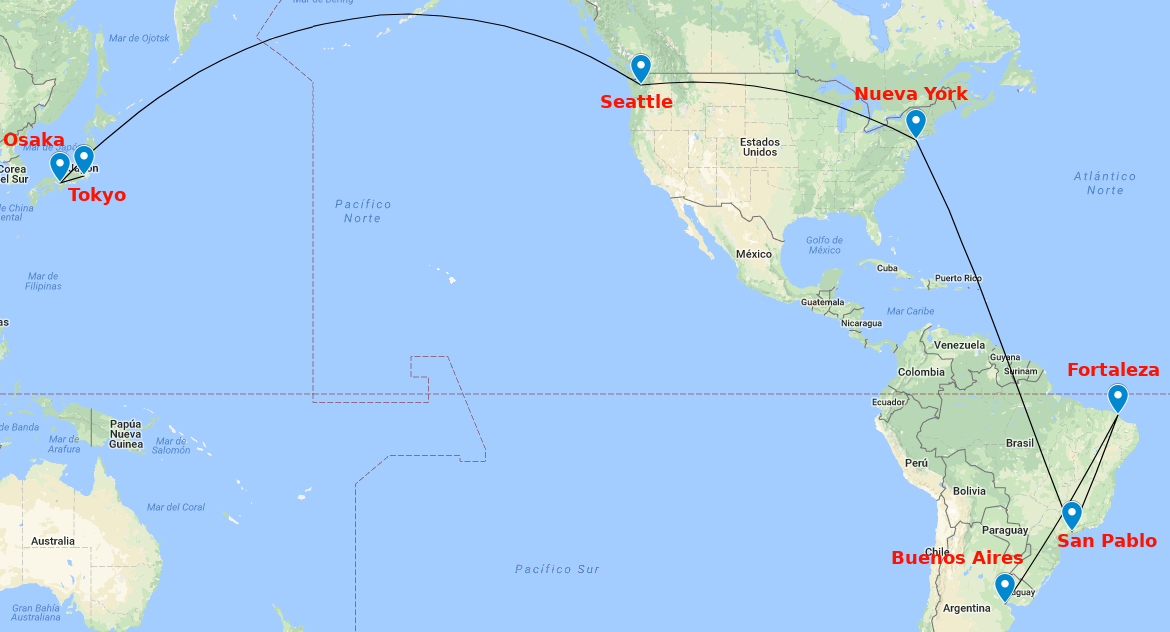
\includegraphics[width=\textwidth]{tokyo.png}
\caption{Mapa de resultados para la Universidad de Tokyo. Corregimos la ubicación del salto número 7.}
\label{mapa1}
\end{figure}

En la figura \ref{diff1} se puede ver que la mayor diferencia se da en el salto 16, pero a la vez el mayor salto negativo se da en el salto 17. De esto deducimos que probablemente haya varios saltos posibles en esta zona, y la ruta elegida por la herramienta es una mezcla de alguna de estas. Esto ocurre cuando los paquetes están en Japón. El resto de los puntos no muestran una tendencia definida (ni creciente ni decreciente).

\begin{figure}[H]
\centering
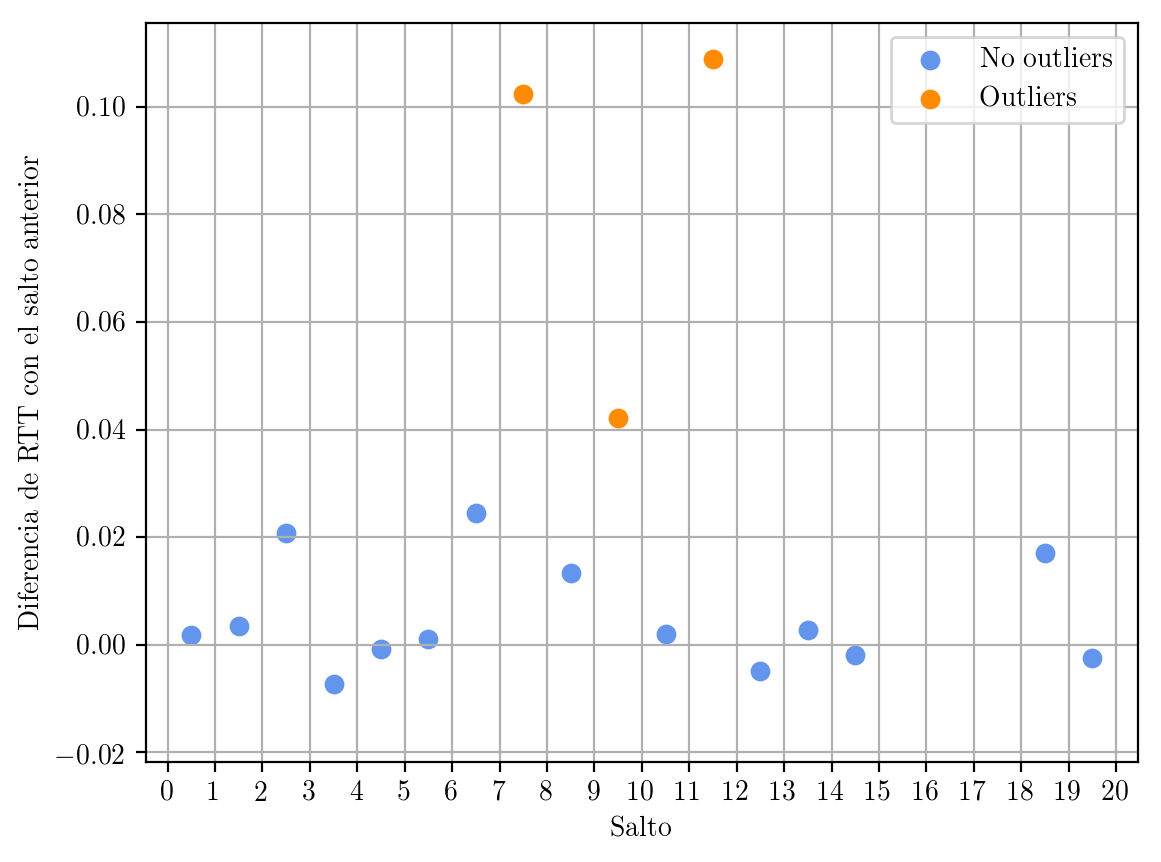
\includegraphics[width=0.6\textwidth]{tokyo1.png}
\caption{Gráfico de diferencias de RTT en función de cada salto.}
\label{diff1}
\end{figure}

De la figura \ref{sdev1} vemos que los puntos están muy dispersos, lejos del 0 de $x$ (que representa el promedio). Por eso el método de Cimbala resultó con muchos outliers.

\begin{figure}[H]
\centering
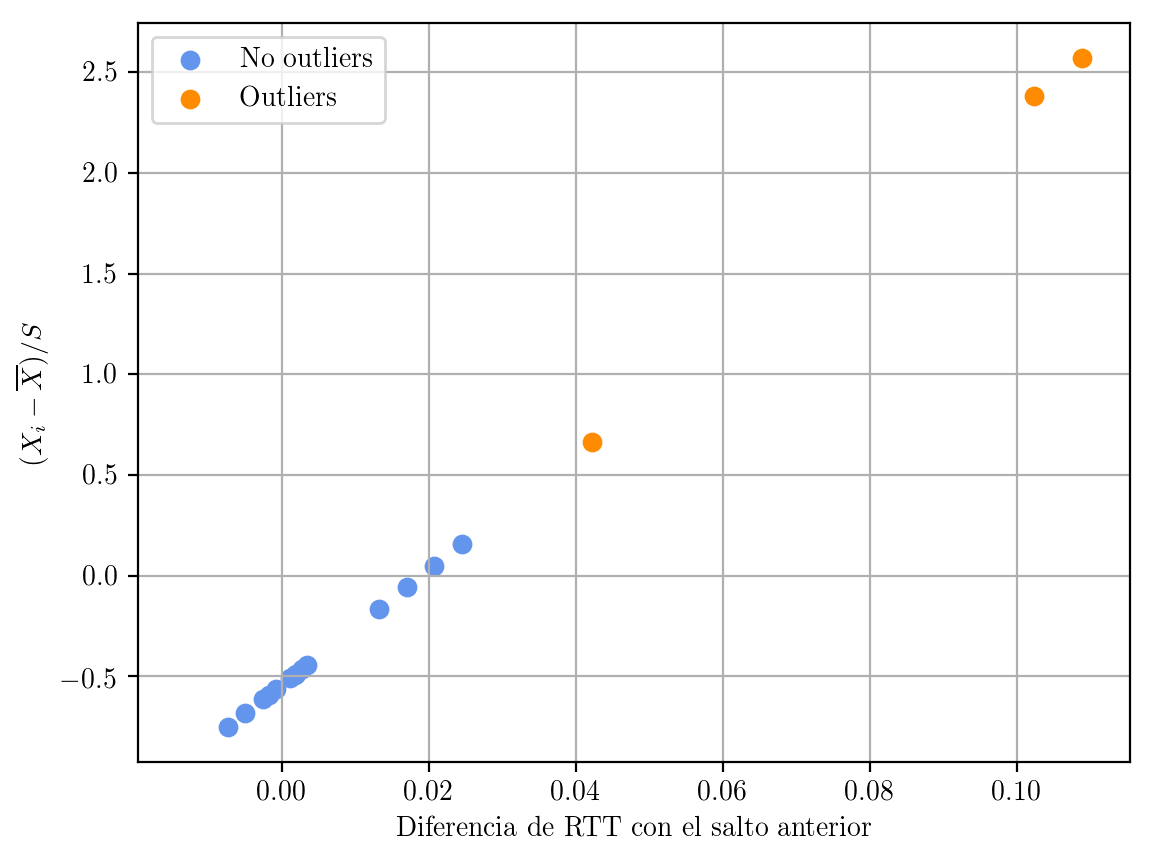
\includegraphics[width=0.6\textwidth]{tokyo2.png}
\caption{Gráfico de $\frac{X_i - \bar{X}}{S}$ en función de las diferencias de RTT.}
\label{sdev1}
\end{figure}

Atribuimos los falsos positivos en Argentina a la diferencia de la velocidad de conexión con el resto del mundo. De acuerdo al reporte del estado de internet de Akamai \cite{akamai} nuestro país tiene baja velocidad promedio de internet, como se muestra en la figura \ref{speed}. Como estamos usando los RTT para calcular los saltos, no podemos saber si un RTT entre saltos más grande se debe a mayor distancia o a menor velocidad. Esto posibilita los falsos positivos.

En cuanto a Japón, vemos en la figura \ref{speed} que su velocidad de conexión es mucho más alta que el promedio. Pero como fue mencionado antes, en esa zona probablemente haya rutas alternativas internas y el criterio elegido puede mezclarlas entre sí, causando falsos positivos.

\begin{figure}[H]
\centering
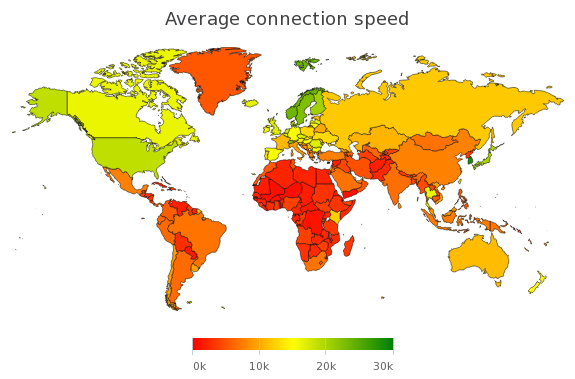
\includegraphics[width=0.7\textwidth]{speed.png}
\caption{Velocidades promedio de internet en el mundo.}
\label{speed}
\end{figure}
